\documentclass[sigconf]{acmart}

\usepackage{booktabs} % For formal tables

\usepackage{amsmath}
\usepackage{float}
\usepackage{hyperref}
\usepackage{listings}
\usepackage{algorithm}
\usepackage[noend]{algpseudocode}
\usepackage{graphicx}
\usepackage{courier}
\usepackage{float}
\usepackage{color}
\usepackage[margin=10pt,font=small,labelfont=bf,
  labelsep=endash]{caption}
\usepackage{ulem}

\usepackage{syntax} % for writing BNF grammar

\usepackage{forest}
\usepackage{framed}

\usepackage{tikz}
\usetikzlibrary{matrix}
\usetikzlibrary{shapes.multipart}
\usetikzlibrary{patterns}
\usetikzlibrary{positioning,fit,calc}
\usetikzlibrary{decorations.pathmorphing}
\usetikzlibrary{decorations.pathreplacing}
\usetikzlibrary{quotes}
\usetikzlibrary{graphs}
\usetikzlibrary{arrows.meta}
\usetikzlibrary{shapes}
% \usetikzlibrary{graphs,graphdrawing}
% \usegdlibrary{layered}
% \usetikzlibrary{graphdrawing,graphs,calc}
% \usegdlibrary{layered}

\usepackage{smartdiagram}

% \usetikzlibrary{external}
% \tikzexternalize % activate!
% \tikzset{external/force remake}

%% To generate figure, uncomment above three lines, and execute:
%% pdflatex -shell-escape helium.tex

\usepackage{csvsimple}
\usepackage{multirow}


\lstset{basicstyle=\footnotesize\ttfamily,breaklines=true}
% \lstset{frame=b}
\lstset{float,floatplacement=H,captionpos=b}
% \lstset{numbers=left}
\lstset{language=C}
\lstset{showstringspaces=false}
\lstset{breakindent=10pt}
% \lstset{framextopmargin=10pt}
% \lstset{framextopmargin=50pt,frame=t}
% \lstset{float=htb,language=C,frame=single, basicstyle=\small, stringstyle=\ttfamily}
% \lstset{escapeinside={(*@}{@*)}}
% \usepackage{xcolor}
\lstdefinestyle{base}{
  language=C,
  emptylines=1,
  breaklines=true,
  aboveskip=0em,
  belowskip=0em,
  % float,
  % floatplacement=H,
  basicstyle=\footnotesize\ttfamily\color{black},
  moredelim=**[is][\color{blue}]{@}{@},
  moredelim=**[is][\color{purple}]{~1}{~1},
  moredelim=**[is][\color{brown}]{~2}{~2},
  moredelim=**[is][\color{gray}]{~3}{~3},
  moredelim=**[is][\color{orange}]{~4}{~4},
  moredelim=**[is][\color{violet}]{~5}{~5},
}
\lstdefinestyle{graycode} {
  language=C,
  emptylines=1,
  breaklines=true,
  basicstyle=\footnotesize\ttfamily\color{gray!50},
  moredelim=**[is][\color{blue}]{@}{@},
}
\lstset{style=base}




\begin{document}

\title{Test}



\begin{figure*}
  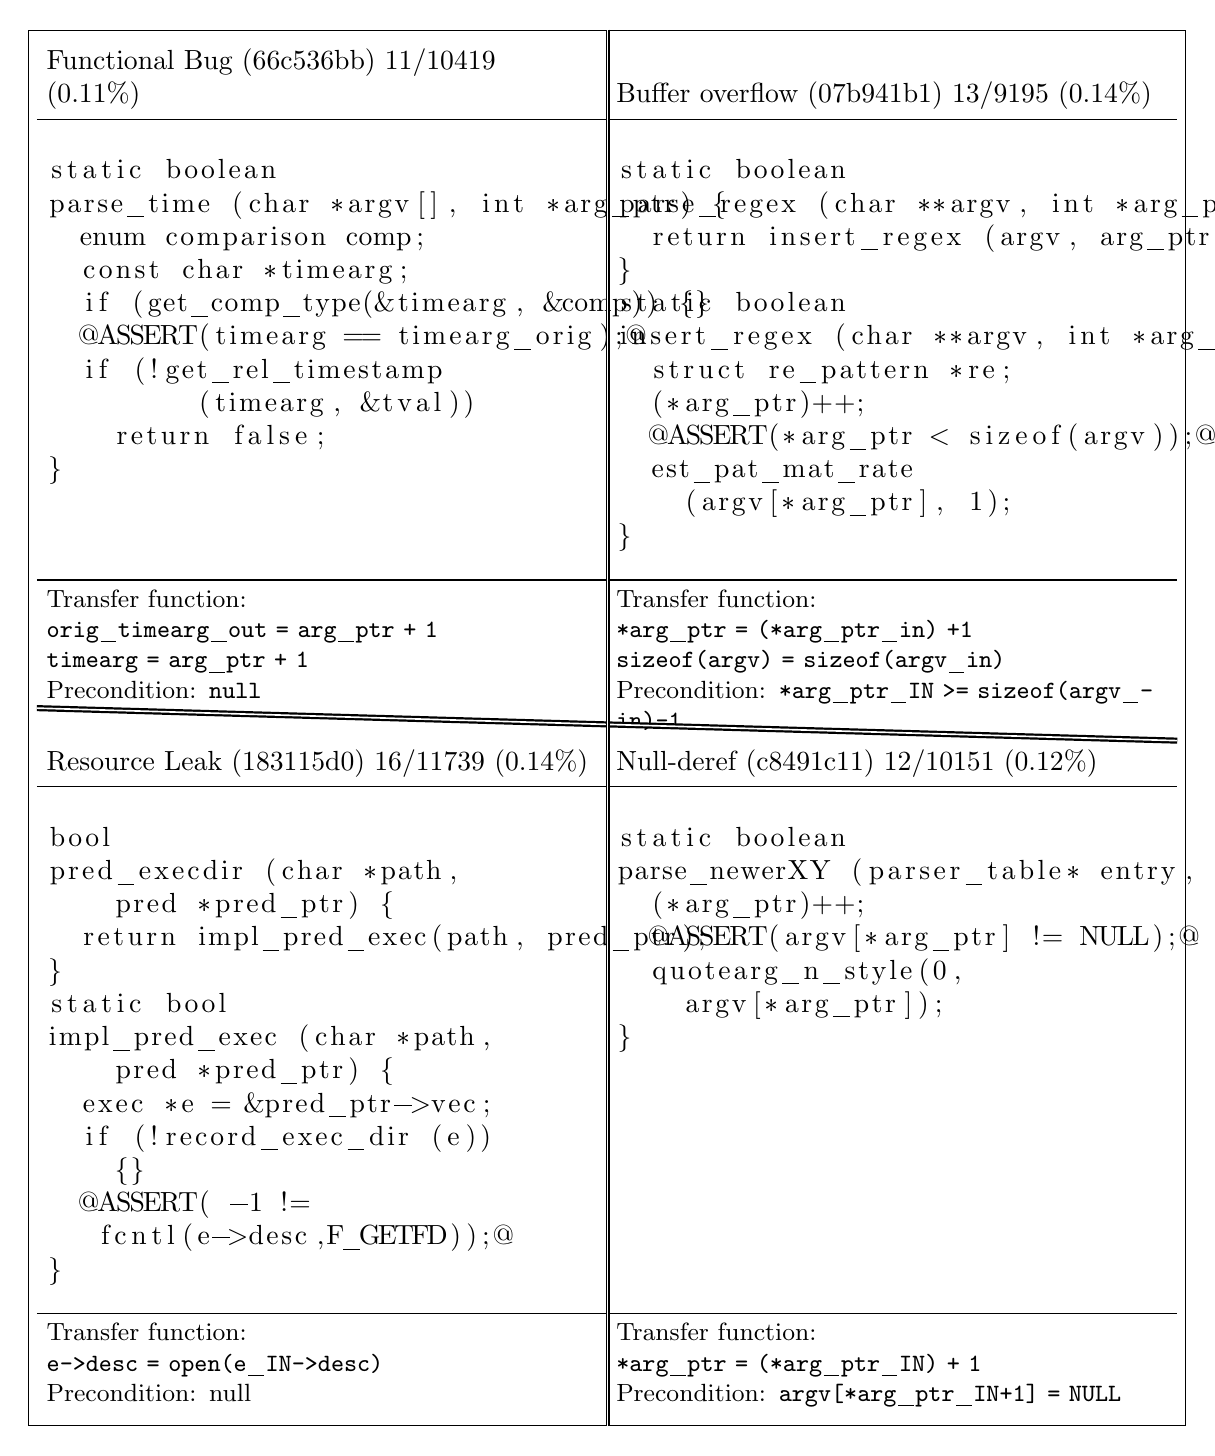
\begin{tikzpicture}
    \matrix (m) [
      draw,
      matrix anchor=north,
      every node/.style={
        % draw,
        anchor=north west, text width=7cm}] {
      \node (c1) ["Functional Bug (66c536bb) 11/10419 (0.11\%)"]{
        \begin{lstlisting}
static boolean 
parse_time (char *argv[], int *arg_ptr) {
  enum comparison comp;
  const char *timearg;
  if (get_comp_type(&timearg, &comp)) {}
  @ASSERT(timearg == timearg_orig);@
  if (!get_rel_timestamp
         (timearg, &tval))
    return false;
}
\end{lstlisting}
      };&
      \node (c2) ["Buffer overflow (07b941b1) 13/9195 (0.14\%)"] {
        \begin{lstlisting}
static boolean
parse_regex (char **argv, int *arg_ptr) {
  return insert_regex (argv, arg_ptr, entry);
}
static boolean
insert_regex (char **argv, int *arg_ptr) {
  struct re_pattern *re;
  (*arg_ptr)++;
  @ASSERT(*arg_ptr < sizeof(argv));@
  est_pat_mat_rate
    (argv[*arg_ptr], 1);
}
\end{lstlisting}
      };\\
      \node (f1) [font=\small]{
        Transfer function:\\
        \texttt{orig_timearg_out = arg_ptr + 1}\\
        \texttt{timearg = arg_ptr + 1}\\
        Precondition: \texttt{null}\\
      };&
      \node (f2) [font=\small] {
        Transfer function:\\
        \texttt{*arg_ptr = (*arg_ptr_in) +1}\\
        \texttt{sizeof(argv) = sizeof(argv_in)}\\
        Precondition: \texttt{*arg_ptr_IN >= sizeof(argv_in)-1}
      };\\
      \node (c3) ["Resource Leak (183115d0) 16/11739 (0.14\%)"] {
        \begin{lstlisting}
bool
pred_execdir (char *path,
    pred *pred_ptr) {
  return impl_pred_exec(path, pred_ptr);
}
static bool
impl_pred_exec (char *path,
    pred *pred_ptr) {
  exec *e = &pred_ptr->vec;
  if (!record_exec_dir (e))
    {}
  @ASSERT( -1 !=
   fcntl(e->desc,F_GETFD));@
}
\end{lstlisting}
      };&
      \node (c4) ["Null-deref (c8491c11) 12/10151 (0.12\%)"] {
        \begin{lstlisting}
static boolean
parse_newerXY (parser_table* entry, char **argv, int *arg_ptr) {
  (*arg_ptr)++;
  @ASSERT(argv[*arg_ptr] != NULL);@
  quotearg_n_style(0,
    argv[*arg_ptr]);
}
\end{lstlisting}
      };\\
      
      \node (f3) [font=\small] {
        Transfer function:\\
        \texttt{e->desc = open(e_IN->desc)}\\
        Precondition: null\\
      };&
      \node (f4) [font=\small] {
        Transfer function:\\
        \texttt{*arg_ptr = (*arg_ptr_IN) + 1}\\
        Precondition:
        \texttt{argv[*arg_ptr_IN+1] = NULL}\\
      };\\
    };
    \draw [] (c1.north west) -- (c2.north east);
    \draw [] (c3.north west) -- (c4.north east);
    % \draw [double, thick] (s1.north west) -- (s4.north east);
    \draw [double, thick] (f1.south west) -- (f2.south east);
    \draw [] (f1.north west) -- (f2.north east);
    \draw [] (f3.north west) -- (f4.north east);
    % \foreach \x in {1,2,3}
    % \draw [dotted, thick] (c\x.north east |- m.north) -- (f\x.south east |- m.south);
    \draw [double] (c1.east |- m.north) -- (f3.east |- m.south);
  \end{tikzpicture}
  \caption{Bug signature of four types. Programs and revisions in GNU
    findutils. Code simplied to fit in space, e.g. remove parameters,
    rename identifiers}
\end{figure*}

\end{document}
